%\pagestyle{fancy}
\chapter{Results}
\label{ch:Results}

\section{Evaluation concept}
\todoin{\begin{itemize}
    \item Explanation of scores etc
    \item Taking average for multiple ramps but also one single ramp
\end{itemize}}



\section{Ramp metering? (\glsentrytext{imu})}
\todoin{\begin{itemize}
    \item How well do different \gls{imu} methods work...
    \item ... at ramp detection
    \item ... at ramp distance measuring
    \item ... at angle estimation
\end{itemize}}



\section{Ramp detection (\glsentrytext{lidar} and camera)}
\todoin{\begin{itemize}
    \item Confusion matrix or similar (false negatives could be hard (e.g. curve))
    \item Estimated angle and distance compare to ground truth
    \item Do downwards ramp work?
    \item Camera \gls{lidar} projection for nice visualization
    \item Something about camera
\end{itemize}}

\begin{figure}[htbp]
    \centering
    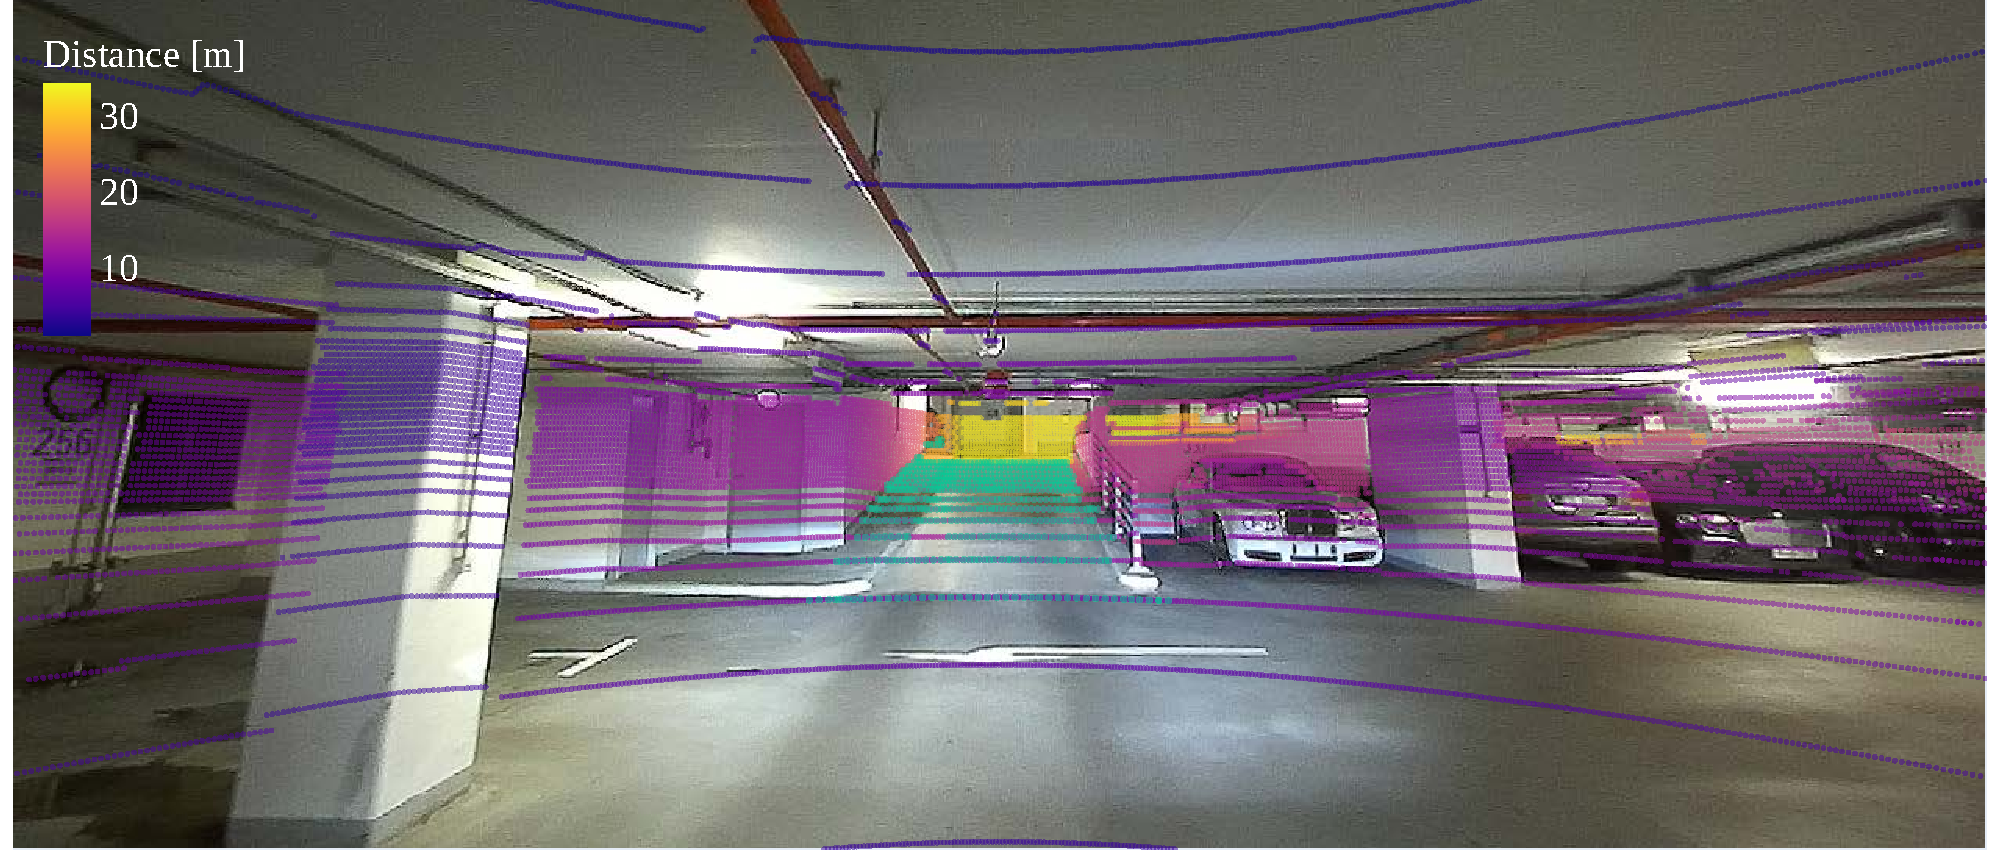
\includegraphics[width=1\linewidth]{points_projection.pdf}
    \caption{Ramp detection in action}
\end{figure}

\begin{figure}[htbp]
    \centering
    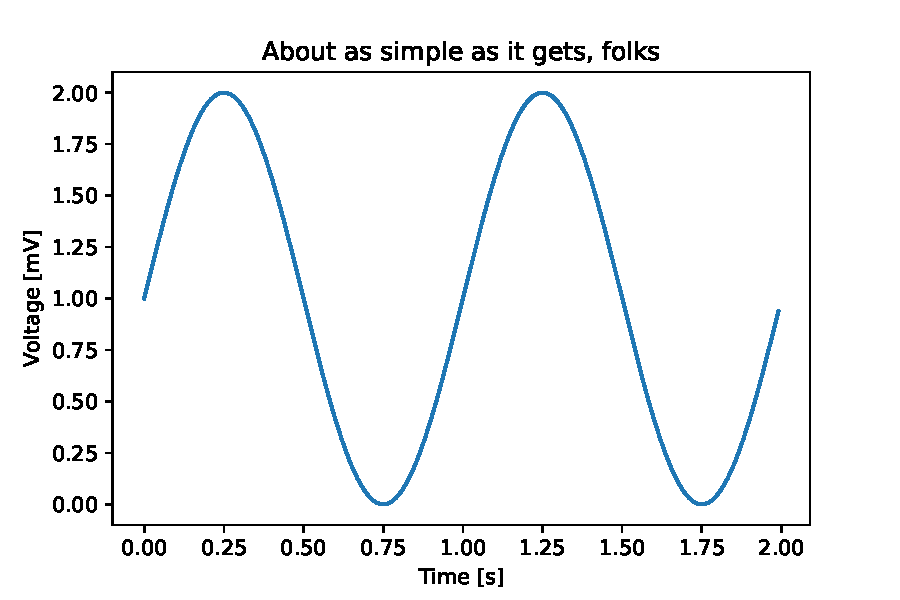
\includegraphics[width=0.7\linewidth]{matplotlib.pdf}
    \caption{Standard matplotlib}
\end{figure}

\begin{figure}[htbp]
    \centering
    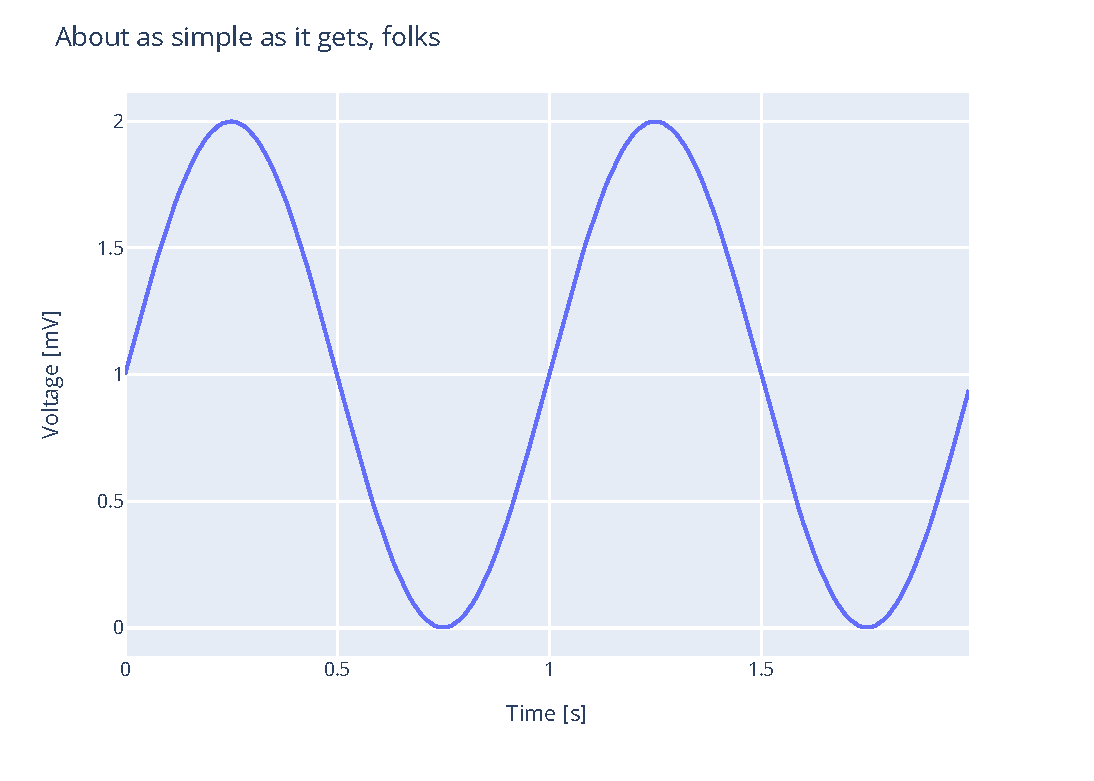
\includegraphics[width=0.7\linewidth]{plotly.pdf}
    \caption{Standard plotly}
\end{figure}